\chapter{Istniejące sposoby wydobywania kolokacji opisane w literaturze}
Znaczna część dotychczasowych prac nad wydobywaniem kolokacji ogranicza się w dużym stopniu tylko do badania wyrażeń dwuelementowych.
Jeśli natomiast badane są kolokacje o większej liczbie elementów, często stosuję się podejścia wykorzystujące uproszczone modele statystyczne.
Dodatkowo sposoby wyszukiwania jednostek wielowyrazowych w tekstach języka polskiego nie były do tej pory często badane, zwłaszcza w kontekście wyrażeń o długości większej niż dwa.
\par
Przykładem pracy która dotyczy innego zagadnienia niż kolokacje, ale traktującej także o ekstrakcji wyrażeń dwuelementowych z tekstów języka polskiego, jest praca magisterska Aleksandra Buczyńskiego \cite{buczynski}.
\par
W tej części niniejszej pracy, na podstawie literatury skupimy się na opisie metod wydobywania wyrażeń dwuelementowych z niepolskojęzycznych tekstów, (głównie anglojęzycznych).
Zaznaczyć należy jednak, że omówione tutaj metody mogą być także stosowane dla języka polskiego i innych języków słowiańskich i o bogatej fleksji.
Ponadto dla lepszego zrozumienia przedstawianych metod podawane będą przykłady ich zastosowania przy zadaniu ekstrakcji bi-gramów, a w dalszej części tego rozdziału zamieszczone zostanie także wprowadzenie do miar mogących posłużyć do wydobywania kolokacji wieloelementowych - dłuższych niż dwie składowe.


\section{Metoda zliczania}

\subsection{Opis metody}
Pierwsza z przytoczonych w tym rozdziale metod ekstrakcji kolokacji jest jednym z najprostszych i dość naiwnych sposobów polegającym na wykorzystaniu podstawowej cechy opisującej słowa w korpusie - ich częstości.
Cecha ta określa ile razy w rozważanych danych tekstowych wystąpił konkretny token, gdzie ten może być rozumiany jako pojedyncze słowo, cały n-gram lub inne zestawienie określonej liczby wyrazów.

\par
Technika zliczania korzysta z założenia mówiącego o tym, że jeśli dany zestaw wyrazów występuje w tekście w określonej kolejności bardzo często, częściej niż inne tego typu zbiory słów, to jest to znak, że rozważane zestawienie ma pewne specjalne znaczenie, może nieść ze sobą interesujące informacje i należy zwrócić na nie uwagę \cite[str. 153]{mit}.

\par
Niestety w tym podejściu pojawia się problemem związany z częstościami słów.
Przy zliczaniu liczby wystąpień danych wyrazów lub ich zbiorów w konkretnym zestawie tekstów, będących podzbiorem wszystkich tekstów języka, dokonuje się na nim pewnej generalizacji.
Polega ona na tym, że jeśli w rozważanym tekście dany zbiór wyrazów został uznany za jednostkę wielowyrazową, to z punktu widzenia całego języka także będzie uważany za kolokację.
Pamiętać trzeba, że generalizacja jest jedynie przybliżeniem rzeczywistości, ponieważ powstała zaledwie na podstawie pewnej próbki losowej tekstów tego języka.
Może ona być pożądana, o ile jest poprawna -- reprezentacyjna dla całego języka, jednak bardzo trudnym zadaniem jest jej utworzenie na podstawie tylko części tekstów rozważanego języka \cite[str. 20]{evert}.

\par
Mimo problemu związanego z niepewnością generalizacji warto przedstawić tę metodę i osiągane przez badaczy wyniki przy jej wykorzystaniu, ponieważ może być to dobry punkt odniesienia do rozważań nad innymi sposobami wydobywania kolokacji.
Dzięki przybliżeniu tej metody pozyskać można podstawową wiedzę na temat ekstrakcji kolokacji, a ponadto obserwacje badaczy mogą dostarczyć wielu cennych informacji.

\par
Metoda częstości polega na zliczeniu wszystkich wystąpień każdego z tokenów i wykorzystaniu poniższego założenia, wspomnianego wcześniej:

\begin{center}
Jeśli dane słowa występują w tekście razem bardzo często to znaczy, że dany zestaw wyrazów spełnia jakąś ważną funkcję, której nie można w prosty sposób wyjaśnić jako funkcji będącej jedynie wynikiem kombinacji tych wyrazów \cite[str. 153]{mit}.
\end{center}

Jeśli to założenie jest spełnione, dane współwystępowanie wyrazów powinno zostać uznane za kolokację lub przynajmniej za ciekawego kandydata na takie zaklasyfikowanie.


\subsection{Wyniki metody}
Wyniki badań przeprowadzonych przez Manninga i Schütze \cite[str. 154]{mit} obrazują bardzo złe wyniki metody i wskazują słaby jej punkt.
Powodem niezadowalających wyników jest przewaga częstości występowania słów funkcyjnych języka oraz bi-gramów z nich złożonych, głównie anglojęzycznych zwrotów \emph{of the} oraz kilku innych współwystąpień z wyrazem \emph{the}.
Spośród dwudziestu najczęściej występujących dwuelementowych zwrotów, aż dziewiętnaście to właśnie wyrażenia funkcyjne języka angielskiego, które nie są kolokacjami.
Tylko jedna pozycja z listy może zostać uznana za wyrażenie wielowyrazowe i jest to nazwa miasta - \emph{New York} \cite[154]{mit}.
Jednak jakość wyników tej metody okazała się zgodna z przewidywaniami autorów \cite{mit} - zwykłe wybieranie najczęściej współwystępujących wyrazów nie prowadzi do interesujących wyników w dziedzinie badania sposobów wydobywania kolokacji \cite[str. 153]{mit}.


\subsection{Rozszerzenie algorytmu o filtr części mowy}
Manning i Schütze w swojej pracy przedstawili sposób na znaczną poprawę jakości wyników poprzez zastosowanie prostej heurystyki w postaci kilku filtrów opartych o części mowy.
Pomysł na taką technikę poprawy wyników został zaczerpnięty z pracy Justesona i Katza wspomnianej w literaturze \cite[str. 154]{mit}.
Kandydaci na wyrażenia wielowyrazowe, którzy nie spełniali określonych wzorców składniowych części mowy, a konkretnie postaci przymiotnik-rzeczownik lub rzeczownik-rzeczownik \cite[str. 155]{mit} byli wykluczani z listy potencjalnych kolokacji.


\subsection{Wyniki po zastosowaniu filtra}
Wyniki po filtrowaniu okazały się znacznie lepsze od tych, jakie uzyskano metodą bez filtrowania, ponieważ tym razem z dwudziestu par wyrazów, które wystąpiły najczęściej w badanych tekstach autorzy nie zakwalifikowaliby jedynie trzech bi-gramów jako niekompozycyjnych \cite[str. 155]{mit}.

\par
Dużą zaletą tej heurystyki jest fakt, że można ją zastosować także w połączeniu z innymi metodami wydobywania kolokacji, także z tymi, które zostaną przez autora niniejszej pracy przytoczone w dalszej części rozdziału.

\par
Zastosowanie takiego filtrowania wymaga jednak dziedzinowej wiedzy lingwistycznej lub badań w celu oceny, które połączenia części mowy mogą ewentualnie tworzyć ciekawych kandydatów na wyrażenia wielowyrazowe, a które raczej nie mają ku temu tendencji.
Jako przykład badań mogących pomóc w doborze filtrów dla języka czeskiego będącego bardziej skomplikowanym w analizie niż język angielski, można podać artykuł autorstwa Pavla Peciny \emph{Reference Data for Czech Collocation Extraction}, prezentujący częstość występowania par słów wraz z ich częściami mowy w zbadanych przez niego zestawach danych \cite{pecina_resource}.

\par
Trudnym zadaniem może być też wyznaczenie filtrów i podjęcie decyzji, których należy użyć w procesie wydobywania kolokacji, a których stosować nie warto.
Zwiększanie liczby filtrów może zaowocować wzrostem kompletności, ale spadkiem precyzji, zwłaszcza kiedy dane zestawienia części mowy w konkretnym filtrze będą rzadko tworzyć kolokacje w stosunku do liczby wszystkich wyrażeń przez nie generowanych.


\subsection{Wnioski}
Manning i Schütze zwracają uwagę na istotny wniosek płynący z badań nad tą prostą metodą wydobywania kolokacji.
Zauważają, że nawet użycie nieskomplikowanych technik ilościowych wspieranych przez niewielką wiedzę lingwistyczną może dać wręcz niespodziewanie dobre wyniki w zadaniu automatycznej ekstrakcji wyrażeń wielowyrazowych \cite[str. 155, 157]{mit}.



\section{Wariancja i odległość słów}

Metoda zliczania wzbogacona o filtrowanie oparte o części mowy słów sprawdza się nad wyraz dobrze dla języka angielskiego przy wydobywaniu kolokacji ciągłych, ale niestety ta technika nie sprawdzi się tak dobrze przy ekstrakcji jednostek wielowyrazowych o zmiennym szyku lub z przerwami pomiędzy składowymi kolokacji -- wyrażeniami nieciągłymi \cite[str. 157]{mit}.
Sposobem, który stanowi pomoc w radzeniu sobie z tym problemem jest metoda oparta o średnią odległość słów oraz wariancję i odchylenie standardowe odległości.

\subsection{Opis metody}
Technika wykorzystuje okno przesuwne o określonej długości oznaczającej rozmiar otoczenia aktualnie rozpatrywanego słowa w korpusie.
Mówiąc inaczej okno przesuwne zawiera w sobie \emph{słowo przetwarzane} i jego kontekst.
Długość okna jest liczbą całkowitą określającą liczbę wyrazów po każdej ze stron słowa przetwarzanego, które w danym momencie będzie rozważane \cite[str. 158]{mit}.
Dla przykładu, zastosowanie okna o długości dwóch wyrazów, przesuwanego za każdym razem o jedno słowo w przykładowym zdaniu \emph{Niestety trzeba przyznać, że pogoda dzisiaj nam nie dopisała} oraz przy pominięciu znaków interpunkcyjnych spowoduje rozpatrzenie kolejno takich n-gramów jak \textit{\textbf{Niestety} trzeba przyznać}, \textit{Niestety \textbf{trzeba} przyznać że}, \textit{Niestety trzeba \textbf{przyznać} że pogoda}, \textit{trzeba przyznać \textbf{że} pogoda dzisiaj} i tak dalej, aż okno zostanie przesunięte do końca aktualnie rozważanego zdania.
Słowa wytłuszczone to te, na które ustawione było okno przesuwne w danej iteracji -- słowo przetwarzane, aktualnie rozważane w korpusie \cite[str. 158]{mit}.
Przypadek braku wystarczającej liczby słów w oknie może być rozpatrzony dwojako -- można wtedy wziąć pod uwagę mniejszą liczbę wyrazów do rozważań lub ominąć ten fragment tekstu i przesunąć okno dalej.

\par
Dla każdego przyłożenia okna tworzeni są kandydaci na kolokacje o konkretnej długości wyrażonej w liczbie słów.
Dla uproszczenia ograniczmy rozważania do wyrażeń dwuelementowych.
Kandydaci tworzeni są w taki sposób, że kreowane i zapamiętywane są wszystkie możliwe kombinacje o długości dwóch słów spośród znajdujących się aktualnie w granicach okna.
Istotne jest, aby ustalić czy po dodaniu kandydatów z jednego przyłożenia okna powielać ich po przesunięciu tego okna, czy jedynie dodać pary powstałe dzięki nowemu słowu w oknie, co wydaje się bardziej rozsądnym posunięciem.

\par
Przykład tworzenia kandydatów na kolokacje w obrębie jednego przyłożenia okna został opisany poniżej.
Rozważmy podane zdanie z wykorzystaniem okna o długości dwóch wyrazów, gdzie tekstem pogrubionym zostało oznaczone słowo przetwarzane -- to, do którego w danym momencie zostało przyłożone okno przesuwne.
Przyjmijmy też przeskok okna równy jednemu wyrazowi -- okno przesuwane jest o jeden wyraz dalej w stosunku do poprzedniej pozycji z każdym nowym przyłożeniem.
\begin{center}
\textit{Zdenerwowało mnie \textbf{Twoje} wczorajsze zachowanie.}
\end{center}
Na podstawie przytoczonego zdania można utworzyć dwadzieścia różnych kombinacji dwuelementowych, a pięć z nich zostało zamieszczonych w poniższej tabeli \ref{sliding_window_example}.

\begin{table}[h!]
\centering
\begin{tabular}{l l l}
	\toprule
	Nr.	& wyrażenie 				& słowa zdania		\\
	\midrule
	1. 	& Zdenerwowało mnie			& pierwsze, drugie	\\
	2. 	& Zdenerwowało Twoje 		& pierwsze, trzecie	\\
	3. 	& Zdenerwowało wczorajsze 	& pierwsze, czwarte	\\
	4. 	& Zdenerwowało zachowanie 	& pierwsze, piąte	\\
	5. 	& mnie Twoje 				& drugie, trzecie	\\
	6.	& \ldots					& \ldots			\\
	\bottomrule
\end{tabular}
\caption[Przykład wykorzystania okna przesuwnego]{Wyrażenia dwuelementowe utworzone z przykładowego zdania za pomocą przykładowego okna przesuwnego.}
\label{sliding_window_example}
\end{table}

\par
Dla każdej kombinacji słów utworzonej we wszystkich przyłożeniach okna przesuwnego na przestrzeni całego korpusu zapamiętywane są odległości pomiędzy wyrazami.
W ten sposób bada się w jakich odległościach od danego słowa występują inne konkretne wyrazy.
Przykładem niech będą trzy wyrażenia: pierwsze \emph{duże czerwone buty}, drugie \emph{buty koloru czerwonego} oraz trzecie \emph{moje ulubione buty czerwone}.
W pierwszym zwrocie odległość słowa \emph{buty} od wyrazu \emph{czerwone} jest równa jeden, ponieważ słowo \emph{buty} wystąpiło zaraz po słowie \emph{czerwone}, natomiast w drugim odległość wyniosła minus dwa słowa, gdyż wyraz \emph{buty} wystąpił przed przymiotnikiem \emph{czerwonego} dodatkowo z jednym wyrazem pomiędzy nimi.
Trzeci termin jest przykładem analogicznym do poprzedniego, odległość słowa \emph{buty} od wyrazu \emph{czerwony} także jest ujemna, ale tym razem równa minus jeden -- w tym przypadku rzeczownik także wystąpił przed przymiotnikiem, jednak bezpośrednio przed nim.
Średnia odległość słowa \emph{buty} od wyrazu \emph{czerwone} będzie zatem równa: 

$$ \bar{d} = \frac{1}{3}(1 + (-2) + (-1)) = -\frac{2}{3} $$

Natomiast wariancja na podstawie \cite[str. 159]{mit} wyniesie:
\begin{center}
\( s^2 = 
\frac{
	\sum_{i=1}^{n}(d_{i} - \bar{d})^2
}{n - 1} = 
\frac{
	(1 - (-\frac{2}{3}))^2 + 
	(-2 - (-\frac{2}{3}))^2 + 
	(-1 - (-\frac{2}{3})^2)
}{3 - 1} 
\approx \frac{2.78 + 7.11 + 0.11}{2} = 5 \)
\end{center}

\par
W oparciu o zebrane z korpusu informacje o odległościach słów w obrębie każdego przyłożenia okna przesuwnego należy obliczyć średnią odległość występowania wszystkich kombinacji słów, będących kandydatami na kolokacje.
Dodatkowo wymagane jest obliczenie wartości wariancji i odchylenia standardowego $ ( s = \sqrt{s^2} ) $ odległości słów dla każdego z tych kandydatów, a otrzymane w ten sposób wartości posłużą do oceny kandydujących wyrażeń wieloelementowych.
Niska wartość odchylenia standardowego oznacza, że słowa składowe wyrażenia zazwyczaj występują względem siebie w podobnej odległości.
Odchylenie standardowe równe zero należy interpretować jako sytuację, gdy wszystkie wyrazy występują zawsze w tej samej odległości oraz kolejności. \cite[str. 158, 159]{mit}

\par
Średnia odległość słów względem siebie nie niesie informacji pozwalających ocenić, czy rozpatrywany kandydat na wyrażenie wielowyrazowe jest interesujący czy nie jest to prostu wiedza w jakiej średniej odległości dane wyrazy występują względem siebie oraz w jakiej kolejności, chyba że użyta definicja kolokacji nie pozwala na występowanie wyrażeń nieciągłych -- w takiej sytuacji wartość ta może okazać się interesującym dyskryminatorem.
Ze względu na zastosowanie średniej arytmetycznej należy mieć na uwadze długość użytego okna, ponieważ przy niewielkich częstościach nawet pojedyncze wystąpienia obserwacji mocno odstających mogą znacząco zmodyfikować wartości średniej - miara ta jest na nie wrażliwa.
Dlatego z tego powodu podczas oceny wartości średniej odległości międzywyrazowej ważne jest, aby brać pod uwagę także wariancję lub odchylenie standardowe.


\subsection{Wyniki działania algorytmu}
Wyniki otrzymane omawianą metodą mogą być łatwiejsze do oceny w przypadku ich wizualizacji za pomocą prostych wykresów.
Manning i Schütze w swojej pracy zamieścili trzy wykresy odnoszące się do trzech różnych anglojęzycznych wyrażeń: \emph{strong opposition}, \emph{strong support} oraz \emph{strong for}.
Warto wspomnieć, że badania wykonane były z oknem przesuwnym o rozmiarze czterech słów.
Wykresy \ref{manning_shutze_160_1}, \ref{manning_shutze_160_2} oraz \ref{manning_shutze_160_3} zostały wykonane na podstawie danych z wykresów zamieszczonych w pracy wymienionych autorów i są odpowiednikami ich wykresów \cite[str. 160]{mit}.

\begin{figure}[h!]
\centering
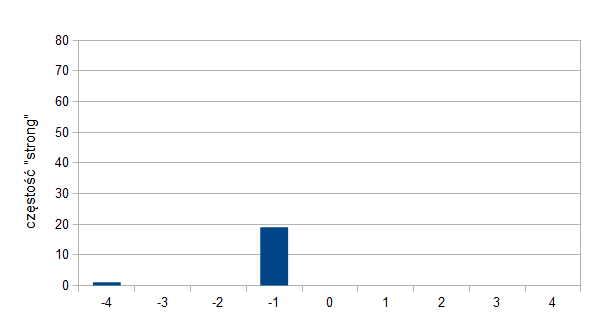
\includegraphics{charts/manning_shutze_160_1}
\caption
	[Słowo \emph{strong} w odniesieniu do słowa \emph{opposition}]
	{
		Słowo \emph{strong} w odniesieniu do słowa \emph{opposition} 
		\begin{displaymath}
			(\bar{d} = -1.15, s = 0.67)
		\end{displaymath}	
		na podstawie wykresów z \cite[str. 160]{mit}
	}
\label{manning_shutze_160_1}
\end{figure}

\par
Pierwszy z wykresów (\ref{manning_shutze_160_1}) składa się w zasadzie z pojedynczego, wysokiego piku, obrazującego, że większość wszystkich wystąpień słowa \emph{strong} razem z \emph{opposition} miało miejsce w odległości minus jeden, czyli słowa te występowały prawie zawsze po sobie w ustalonej kolejności, tworząc zwrot \emph{strong opposition}.
Dodatkowo według Manninga i Schütze wartość odchylenia standardowego jest niska i równa 0.67, a średnia odległość to -1.15 słowa.
Taki wynik, mimo dużego skupienia w okolicy argumentu minus jeden, został spowodowany szumem w danych -- pojedynczym wystąpieniem tej pary słów w odległości równej minus cztery wyrazy \cite[str. 159]{mit}.

\begin{figure}[h!]
\centering 
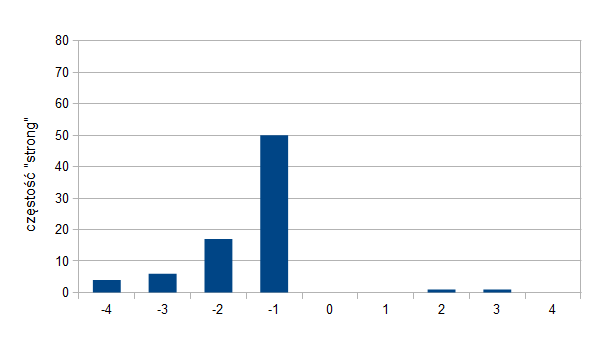
\includegraphics{charts/manning_shutze_160_2} 
\caption
	[Słowo \emph{strong} w odniesieniu do słowa \emph{support}]
	{
		Słowo \emph{strong} w odniesieniu do słowa \emph{support} 
		\begin{displaymath}
			(\bar{d} = -1.45, s = 1.07)
		\end{displaymath}	
		na podstawie wykresów z \cite[str. 160]{mit}
	}
\label{manning_shutze_160_2}
\end{figure}

\par
Na drugim z wykresów (\ref{manning_shutze_160_2}) zamieszczone zostały wyniki, z których wywnioskować można, że słowa \emph{strong} i \emph{support} występowały zazwyczaj w odległości minus jeden od siebie, ale wystąpiło także stosunkowo dużo sytuacji, w których ta odległość była większa, jednak prawie zawsze ujemna.
Zaobserwować można także niemal monotoniczny przebieg wykresu, przy pominięciu mało znaczących, pojedynczych wystąpień w odległościach dwa i trzy.
Zwiększenie zakresu argumentów, dla których występują znaczące wartości określające liczbę wystąpień miało wpływ na wzrost wartości wariancji do poziomu 1.07 \cite[str. 161]{mit}.

\begin{figure}[h!]
\centering
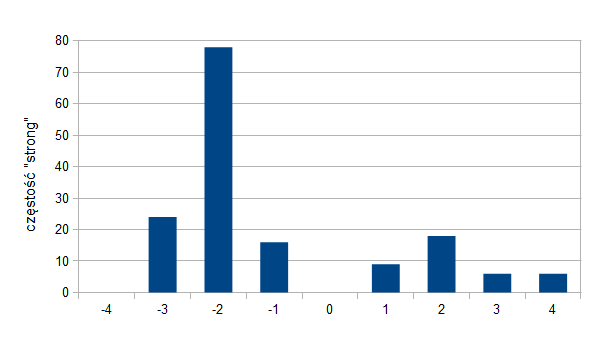
\includegraphics{charts/manning_shutze_160_3}
\caption
	[Słowo \emph{strong} w odniesieniu do słowa \emph{for}]
	{
		Słowo \emph{strong} w odniesieniu do słowa \emph{for} 
		\begin{displaymath}
			(\bar{d} = -1.12, s = 2.15)
		\end{displaymath}	
		na podstawie wykresów z \cite[str. 160]{mit}
	}
\label{manning_shutze_160_3}
\end{figure}

\par
Trzeci wykres (\ref{manning_shutze_160_3}) obrazuje wyniki dla zwrotu niebędącego kolokacją, składającego się z pary wyrazów \emph{strong} oraz \emph{for}.
Wartości na osi rzędnych dla różnych argumentów -- wartości odległości, osiągają znaczące poziomy, nie wykazując żadnej monotoniczności czy skoncentrowania w okolicy jednej z wartości odległości, jak to miało miejsce w przypadku dwóch poprzednich wykresów.
Mimo wysokiej wartości częstości wystąpień dla odległości równej minus dwa (duży pik), taki rozkład wyników spowodował znaczy wzrost wariancji w stosunku do rezultatów poprzednich badań -- odpowiednio ponad trzy- i dwukrotny.
Wysoka wartość wariancji i ocena rozkładu odległości rozpatrywanych wyrazów od siebie spowodowała odrzucenie kandydata \emph{strong for} jako interesującego w kontekście wyrażeń wielowyrazowych \cite[str. 161]{mit}.

\par
Interesującym zestawieniem wyników może być tabela \ref{mean_variance_result_table}, utworzona na podstawie danych z tabeli numer 5.5 w pracy \cite[str. 161]{mit}.
\begin{table}[h!]
\centering
\begin{tabular}{l l l | l | l}
	\toprule
	\textbf{s}	& \textbf{odległość}	& \textbf{częstość}	& \textbf{słowo A}		& \textbf{słowo B} 	\\
	\midrule
	0.43		& 0.97					& 11657				& New					& York				\\
	0.48 		& 1.83					& 24				& previous				& games				\\
	0.15 		& 2.98 					& 46				& minus					& points			\\
	0.49 		& 3.87 					& 131				& hundreds				& dollars			\\
	\midrule
	1.07 		& 1.45 					& 80				& strong				& support			\\
	1.13 		& 2.57 					& 7					& powerful				& organizations		\\
	1.01 		& 2.00 					& 112				& Richard				& Nixon				\\
	1.05 		& 0.00 					& 10				& Garrison				& said				\\
	\midrule
	4.03 		& 0.44 					& 36				& editorial				& Atlanta			\\
	4.03 		& 0.00 					& 78				& ring					& New				\\
	3.96 		& 0.19 					& 119				& point					& hundredth			\\
	3.96 		& 0.29 					& 106				& subscribers			& by				\\
	\bottomrule
\end{tabular}
\caption[Wyniki ekstrakcji kolokacji dla metody wariancji i odległości słów]{Wyniki ekstrakcji kolokacji z zastosowaniem metody opartej o wariancję i odległość słów \cite[str. 161]{mit}.}
\label{mean_variance_result_table}
\end{table}

Cztery pierwsze pozycje tabeli obrazują dobrych kandydatów na kolokacje, których cechuje niska wartość odchylenia standardowego.
Cztery ostatnie wiersze to nieinteresujące w kontekście jednostek wielowyrazowych wyrażenia -- ich odchylenie standardowe jest za wysokie, a dodatkowo średnia odległość wyrazów składowych od siebie jest bliska zeru.
Świadczy to o tym, że owe dwa słowa mogą występować w zasadzie w dowolnej kolejności lub szyku.
Natomiast cztery środkowe pozycje to wyrażenia, których wyrazy występowały w kilku różnych odległościach znaczącą liczbę razy \cite[str. 162]{mit} i są trudniejsze do jednoznacznej oceny niż poprzednie przypadki.


\subsection{Rozszerzenie metody o filtr pików}
Przedstawiona tutaj metoda średniej arytmetycznej i wariancji jest uproszczoną wersją techniki stosowanej przez Smajdę, który opisał ją w 1993 roku \cite{smadja_xtract}.
Wspomniany badacz używał dodatkowo filtru, który odrzucał kandydatów, dla których na wykresie pojawiał się tak zwany płaski pik.
Termin ten określa sytuację, gdy istnieje pewna wysoka wartość dla któregoś z argumentów, ale jednocześnie wartości dla argumentów z jego otoczenia także są znaczącymi liczbami.
Manning i Schütze jako przykład płaskiego piku podali trzeci z poprzednio omawianych wykresów (\ref{manning_shutze_160_3}), dotyczący pary słów \emph{strong for}. 


\subsection{Wyniki dla algorytmu po zastosowaniu filtru}
Przy zastosowaniu tego sposobu wydobywania kolokacji i omówionego filtrowania płaskich pików, Smajda osiągnął dokładność na poziomie osiemdziesięciu procent \cite[str. 162]{mit}.


\subsection{Wnioski}
Wizualizacja danych, tak jak wspomniano wcześniej, może być dodatkowym, pomocnym narzędziem przy ocenie kandydata na kolokację lub próbie wyznaczenia progu wartości wariancji, który będzie używany do odrzucania wyrażeń potencjalnie niebędących jednostkami wielowyrazowymi.
Mimo niewielkiego skomplikowania modelu statystycznego i prostoty filtru Smajda \cite{smadja_xtract} \cite[str. 162]{mit} pokazał, że metoda ta może być skuteczna, a dodatkowo pozwala na ekstrakcję kolokacji nieciągłych co nie było możliwe z wykorzystaniem przedstawionej we wcześniejszej części pracy metody zliczania.


\section{Funkcje asocjacyjne}
Pierwsze dwie omówione metody wykorzystywały częstości słów i konkretnych zestawów wyrazów do oceny wyrażeń w kontekście kandydatury na kolokacje.
Niestety występują trzy problemy związane z uwzględnianiem tylko surowej częstości tokenów w korpusie -- dwa zostały przytoczone przez Everta \cite[str. 20]{evert}, a trzeci przez Manninga i Schütze \cite[str. 162]{mit}.

\par
Pierwszy problem polega na tym, że częste współwystępowanie słów może być czystym przypadkiem, zwłaszcza jeśli częstość tych wyrazów w tekście jest wysoka. 
Fakt ten wpływa negatywnie na jakość oceny kandydatów na jednostki wielowyrazowe z wykorzystaniem metod opartych o zliczanie, więc istotne jest wprowadzanie interpretacji statystycznej częstości \cite[str. 20]{evert}.

\par
Drugi problem to wspomniana już wcześniej generalizacja dla całego języka na podstawie tylko danych wydobytych z pewnego korpusu.
Informacje wyekstrahowane z podzbioru tekstów danego języka, przykładowo tylko z pojedynczego korpusu, mogą okazać się niezrównoważone, niepełne, być jedynie zbliżonymi do tych, które są prawdziwe dla tego języka w ogólności.
Problem ten to ewentualna mała reprezentatywność wykorzystanych danych.

\par
Manning i Schütze zwrócili uwagę na trzeci problem związany z metodą zliczania opartą o odległość i wariancję.
Zauważyli, że wysoka częstość i niska wariancja współwystępowania słów mogą być przypadkowe w sytuacji, kiedy składowe wyrażenia występują często - wtedy oczekiwać można dużej liczby ich współwystąpień tylko ze względu na szansę na takie zdarzenie, a nie na poziom istotności tego wyrażenia w kontekście wydobywania kolokacji \cite[str. 162]{mit}.
Problem polega na tym, że oczekiwanym wynikiem jest informacja nie o tym, czy dany zestaw słów współwystępuje często, tylko czy współwystępuje częściej, niż wynika to jedynie z szansy na takie zdarzenie \cite[162]{mit}.

\par
Próbą rozwiązania wyszczególnionych problemów są różne modele statystyczne.
Mają one udzielać informacji, czy określone obserwacje współwystępowania bytów są czysto przypadkowe, wynikające po prostu z prawdopodobieństwa ich wystąpienia, czy faktycznie istnieją wystarczająco mocne przesłanki statystyczne do tego, aby stwierdzić, że powiązanie pomiędzy nimi faktycznie istnieje i jest istotne. 
Takimi szeroko stosowanymi metodami statystycznymi są \emph{funkcje asocjacyjne} zwane także \emph{miarami asocjacji}, za pomocą których można obliczyć \emph{miarę powiązania} pomiędzy argumentami zadanymi dla funkcji.
Dla przykładu w przypadku bi-gramów argumentami dla tych metod będą pary wyrazów rozważanego kandydata na wyrażenie wielowyrazowe.
Otrzymane za pomocą funkcji asocjacji wyniki, będące liczbami rzeczywistymi, określają stopień powiązania elementów -- to, jak nieprzypadkowe jest ich współwystąpienie. 
Dodatkowo wyniki te mogą posłużyć do utworzenia rankingu i dokonania selekcji kandydatów na kolokacje.

\par
Sytuacja, w której elementy współwystępują częściej niż gdyby były od siebie niezależne, określana jest mianem \emph{asocjacji pozytywnej}, a w przypadku przeciwnym, kiedy występują rzadziej, mianem \emph{asocjacji negatywnej}.
Z powyższym wiąże się ważna cecha funkcji asocjacyjnych w kontekście dostarczanych przez nie wyników -- przynależność do jednej z dwóch następujących grup: \emph{miar jednostronnych} albo \emph{miar dwustronnych}.
Pierwsza z grup zawiera te miary asocjacji, w przypadku których wysoki wynik oznacza silne powiązanie pozytywne, zaś niski -- brak wystarczającego dowodu na powiązanie pozytywne pomiędzy badanymi elementami.
Może występować powiązanie negatywne lub brak powiązania, ale nie da się tego określić na podstawie wyniku działania tej funkcji.
Druga z grup natomiast zawiera miary, których wysoka wartość oznacza silne powiązanie, ale nie daje informacji o tym, jakiego jest ono rodzaju -- pozytywne czy negatywne, a wynik o niskiej wartości to według tej funkcji słabe powiązanie pomiędzy elementami lub jego brak
\cite[str. 20, 21, 75, 76]{evert}.

\par
Większość metod statystycznych omawianych w tej części pracy korzysta z uproszczenia, polegającego na założeniu, że tekst to jedynie zbitka losowo występujących wyrazów ograniczonych przez zasady syntaktyczne języka \cite[str. 6]{pecina_measures}.
Tym samym szansa na wystąpienia danego słowa po dowolnym wyrazie poprzedzającym, nawet takim samym, jest zawsze identyczna na przestrzeni całego tekstu, jednak może być różna dla każdego ze słów.
Chociaż już w 1957 roku Firth zwrócił uwagę osób zajmujących się lingwistyką, że stwierdzenie to jest nieprawdziwe \cite[str. 15]{evert}, i tak jest ono wykorzystywane, niejednokrotnie z powodzeniem, w znacznej części niekontekstowych metod statystycznych, jakimi są miary asocjacyjne.

\par
Funkcje asocjacyjne stosowane są od przynajmniej pół wieku.
Już w roku 1965 dostępnych była pewna liczba funkcji asocjacyjnych, a przez kolejne prawie pięćdziesiąt lat powstało i zostało zbadanych wiele kolejnych. 
Jednak mimo dużej liczby tych miar niewiele z nich zyskało dużą popularność.
Do najbardziej znanych należą \emph{MI (Mutual Information)}, \emph{T-score}, \emph{Log-likelihood} oraz $ Chi^2 $ \cite[str. 21]{evert}.

\par
Pavel Pecina w swoich pracach przedstawił dziesiątki miar asocjacyjnych \cite[str. 3]{coling}\cite[str. 18]{pecina_measures}.
Wszystkie zostały podzielone na sześć grup \cite[str. 2]{coling} -- stanowią one sześć pierwszych pozycji na poniższej liście.
Dodatkowo wyróżnić można kolejne dwie grupy metod ekstrakcji kolokacji -- dwie ostatnie pozycje na liście.

\begin{enumerate}
	\item estymacje współwystąpienia i prawdopodobieństwa warunkowego;
	\item \emph{Mutal Information} i jej pochodne;
	\item testy statystyczne niezależności;
	\item miary z rodziny \emph{likelihood};
	\item zestaw heurystycznych miar asocjacyjnych oraz współczynników zależności;
	\item miary kontekstowe;
	\item \emph{miary mieszane};
	\item \emph{uczenie maszynowe};
\end{enumerate}

Grupy te wraz z przykładami zostały omówione w kolejnych częściach tej sekcji.
Przed ich preyentacjA należy jednak zdefiniować oznaczenia używane we wzorach opisujących te miary:

\begin{itemize}
	\item $ x $ - element \emph{x};
	\item $ \bar{x} $ - element inny niż \emph{x};
	\item $ (x, y, ...) $ - zbiór elementów \emph{x}, \emph{y}, \ldots;
	\item $ p(x) $ - prawdopodobieństwo wystąpienia elementu \emph{x};
	\item $ f(x) $ - częstość elementu \emph{x}, zaobserwowana w zbiorze danych;
	\item $ \hat{f}(x) $ - wartość oczekiwana elementu \emph{x}.
\end{itemize}


\subsection{Współwystąpienia i prawdopodobieństwo warunkowe}
Pierwsza z grup zawiera w sobie trzy podstawowe miary: prawdopodobieństwo współwystąpienia $ p(x, y) $, prawdopodobieństwo warunkowe $ p(x|y) $ oraz odwrócone prawdopodobieństwo warunkowe $ p(y|x) $.
Przytoczone miary to podstawa wykorzystywana w kolejnych rodzinach miar asocjacji.

\subsection{Miary informacji}
Jedną z najpopularniejszych funkcji asocjacyjnych, będących miarą informacji, jest \emph{Mutual Information} wyrażona wzorem\cite[str. 2]{mmi_w11}:

\begin{center}
\( I(X; Y) = \sum_{x \in X} \sum_{y \in Y} p(x, y) log_{2} \frac{p(x, y)}{p(x) * p(y)} \)
\end{center}

Miara ta oblicza ile informacji w jednej zmiennej losowej \emph{X} jest jednoczenie zawarte w drugiej zmiennej losowej \emph{Y} \cite[str. 2]{mmi_w11}.
Natomiast miara \emph{Pointwise Mutual Information} jest wykorzystana do obliczenia poziomu asocjacji dwóch konkretnych wartości zmiennych losowych \emph{X} i \emph{Y}.
Funkcja \emph{PMI} \cite[str. 2]{mmi_w11}, szeroko wykorzystywana w badaniach nad wydobywaniem kolokacji, wyrażona jest wzorem:

\begin{center}
\( pmi(x, y) = log_{2} \frac{p(x, y)}{p(x) * p(y)} \)
\end{center}

Obie z przytoczonych funkcji zostały wykorzystane do budowy innych miar informacji wykorzystywanych w wydobywaniu jednostek wielowyrazowych.


\subsection{Testy statystyczne niezależności}
Jako przykłady miar należących do tej grupy autor niniejszej pracy wybrał trzy: \emph{T-score}, \emph{Z-score} oraz $ Pearson's $ $ X^2 $.
\par
Pierwsza z nich jest częścią \emph{T-testu} \cite[str. 166]{mit}, który składa się trzech głównych kroków: obliczenia wartości dla testu, ustalenia progu wiarygodności i wykonania testu. 
\emph{T-score} natomiast składa się z jednego punktu i jest wykorzystana do tworzenia rankingu, wyliczania wartości zamiast klasyfikacji obserwacji.
Miara \emph{T-score} jest nazywana w literaturze mianem \emph{T-testu} \cite[str. 3]{coling}\cite[str. 18]{pecina_measures}, jednak ze względu na to, że jest jedynie jego częścią polegającą na wyliczeniu wartości, którą można wykorzystać w \emph{T-teście}, w niniejszej pracy będzie nazywana \emph{T-score}.
Wartość tej miary obliczyć można wykorzystując następujący wzór \cite[str. 18]{pecina_measures}:

$$ \frac{f(x, y) - \hat{f}(x, y) }{\sqrt{f(x, y) * (1 - (f(x, y) / N))}} $$

\par
Druga z miar to \emph{Z-score}, która także służy do wyliczenia wartości rankingowej obserwacji, a nie klasyfikacji.
Miara ta w dwóch wcześniej wspomnianych pracach \cite[str. 3]{coling}\cite[str. 18]{pecina_measures} nazywana została już \emph{score}, a nie \emph{test}, jak w przypadku \emph{T-Score}.
Opisana jest za pomocą poniższego wzoru \cite[str. 18]{pecina_measures}:

$$ \frac{f(x, y) - \hat{f}(x, y) }{\sqrt{\hat{f}(x, y) * (1 - (\hat{f}(x, y) / N))}} $$

Różnica pomiędzy miarami \emph{T-score} a \emph{Z-score} to wykorzystanie wartości oczekiwanej zamiast zaobserwowanej w mianowniku wzoru.
Obie te funkcje jednak mają ważną cechę wspólną -- zakładają, że rozkład prawdopodobieństwa w zbiorze danych jest rozkładem normalnym, co w znacznej części przypadków praktycznych nie jest prawdziwe \cite[str. 169]{mit}.

\par
Trzecia z miar to $ Pearson's $ $ X^2 $.
Jej zaletą w stosunku do dwóch poprzednich jest brak założenia co do rozkładu normalnego prawdopodobieństwa w zbiorze danych.
Zamiast tego test zakłada rozkład $ X^2 $ ($ Chi^2 $), który powinien być bardziej odpowiedni do realizacji zadania ekstrakcji kolokacji.
Miara korzysta z tablicy wielodzielnej (ang. contingency table) \cite[str. 169]{mit} w celu porównania wartości obserwowanych z oczekiwanymi i na tej podstawie oceny, czy hipoteza zerowa może zostać odrzucona, a niezerowa przyjęta za prawdziwą.
$ Pearson's $ $ X^2 $ w niniejszej pracy oraz w pracach Pavla Peciny została wykorzystana jako funkcja rankingowa.
Dokonano tego analogicznie jak w przypadku \emph{T-testu}, wyliczono jedynie wartość dla testu, ale on sam nie został wykonany, a uzyskana wartość służy jako wyznacznik pozycji w rankingu.
Wzór funkcji jest następujący \cite[str. 18]{pecina_measures}:

$$ \sum_{i, j} \frac{(f_{i, j} - \hat{f}_{i, j})^{2}}{\hat{f}_{i, j}} $$


\subsection{Funkcje z rodziny \protect\textit{likelihood}}
Dwie funkcje z rodziny \emph{likelihood} zostały zaprezentowanych i zbadane w pracach Pavla Peciny \cite[str. 3]{coling}.
Pierwsza z nich została nazwana \emph{Log likelihood ratio} i została zapisana w formie wzoru:

$$ -2 \sum_{i, j} f_{i, j} log \frac{f_{i, j}}{\hat{f}_{i, j}} $$

Druga funkcja jest modyfikacją pierwszej, jest pozbawiona jednego członu i wyrażona wzorem:

$$ -2 \sum_{i, j} \frac{f_{i, j}^2}{\hat{f}_{i, j}} $$

Według Manninga i Schütze \cite[str. 172]{mit} miary z rodziny \emph{likelihood} są lepsze od testów $ Chi^2 $ dla danych rzadkich, jakimi są kolokacje w dużych zbiorach tekstowych. 
Dodatkowo wyniki są bardziej interpretowalne, ponieważ wskazują czy jedna z hipotez jest bardziej prawdopodobna od drugiej.


\subsection{Miary kontekstowe}
Pavel Pecina w swoich pracach \cite[str. 18]{pecina_measures}\cite[str. 3]{coling} prezentuje 24 miary kontekstowe, których jakość także bada.
Miary kontekstowe bazują na kontekstach (otoczeniu) słów i kandydatów na kolokacje.
Wykorzystywane w przedstawionych przez Pavla Pecine miarach są konteksty dwu- oraz jednostronne i na ich podstawie oraz z wykorzystaniem danych o częstościach obliczane są wartości rankingowe.
Miary kontekstowe wykorzystują także informacje pochodzące z otoczenia kandydatów na wyrażenia wielowyrazowe, a nie tylko dane dotyczące ich bezpośrednio (ich częstości).
\par
Praca Peciny i Schlesingera \cite[str. 4]{coling} wskazuje na to, że miara kontekstowa o nazwie \emph{Cosine context similarity in boolean vector space} osiągnęła jeden z dwóch najlepszych wyników spośród wszystkich osiemdziesięciu dwóch sprawdzonych przez Pecinę i Schlesingera funkcji \cite[str. 4]{coling}.
Obrazuje to, że kontekst może być bardzo pomocny przy ocenie kandydatów na kolokacje.


\subsection{Miary mieszane}
Podejście miar mieszanych zostało zaczerpnięte z prac Peciny i Schlesingera \cite{coling} oraz Anca Dinu, Liviu P. Dinu, Ionut T. Sorodoc \cite{aggregation}.
Pomysł przedstawiony w drugiej z prac polega na wygenerowaniu zestawu rankingów dla różnych miar asocjacyjnych, a następnie opcjonalnym wykonaniu ich przepunktowania, polegającego na zachowaniu kolejności w rankingu, ale zmianie wartości dla każdej z pozycji.
Przykładowymi miarami przepunktowania rankingów są \emph{Rank distance} i \emph{Borda score} \cite[str. 2]{aggregation}.
Kiedy rankingi są gotowe należy poddać je agregacji w celu wygenerowania pojedynczego, finalnego rankingu, który jest także wynikiem algorytmu.
\par
Pavel Pecina wykorzystuje natomiast miary mieszane w innym celu -- opisanym w podrozdziale 3.3.8.


\subsection{Uczenie maszynowe}
Praca Peciny i Schlesingera \cite{coling} pokazuje sposób na wykorzystanie miar asocjacyjnych w celu wygenerowania cech dla algorytmów maszynowego uczenia i regresji liniowej.
\par
Proces generowania cech ma trzy krotki.
Pierwszy z nich to dobór miar asocjacyjnych, które zostaną wykorzystane jako składowe generatora cech do wykorzystania w procesie maszynowego uczenia.
Pavel Pecina wskazuje \cite{coling}, że jest to krok istotny, ze względu na to, iż wiele miar dzieli ze sobą w części te same informacje, a tym samym wykorzystanie niektórych z nich nie powoduje uzyskania dużo lepszych wyników.
Badacz pokazał, że można osiągnąć podobne jakościowo wyniki redukując liczbę dobranych miar asocjacyjnych z 82 do 17 przy zachowaniu około 95\% ich całkowitej wariancji.
Z kolei jedynie 42 miar powoduje utrzymanie poziomu w okolicy 99.9\% \cite[str. 7]{coling}.
Dodatkowo Mariusz Paradowski w swojej pracy \cite{paradowski_beta} zbadał część funkcji asocjacyjnych i wykazał, które z nich są ze sobą skorelowane i w efekcie generują równoważne rankingi.
Polega to na zachowaniu takiej samej kolejności pozycji w różnych rankingach, ale przy ewentualnej różnicy oceny danych bytów na poszczególnych pozycjach.
Informacje te mogą posłużyć do lepszego doboru miar w procesie tworzenia cech dla algorytmów maszynowego uczenia.

\par
Drugi krok generacji cech polega na wykorzystaniu miar asocjacyjnych dla każdego badanego kandydata na kolokacje.
Efektem tego działania jest jeden wektor dla każdej krotki, a każda pozycja tego wektora przechowuje wynik jednej z funkcji asocjacyjnych.
Dodatkowo jeden z jego elementów przechowuje informację, o tym czy kandydat jest kolokacją czy nie -- informacja ta jest wykorzystywana w procesie uczenia nadzorowanego.
W pracy Peciny i Schlesingera klasa jest dwuwartościowa, ale wydaje się, że nic nie stoi na przeszkodzie, aby przypisać jej więcej możliwych wartości.
Przykład wektora został zamieszczony poniżej:
$$ wektor\_cech = [x_{1}, x_{2}, ..., x_{n}, klasa], gdzie: $$
\begin{enumerate}
	\item $ x_{i} $ - wynik dla miary \emph{i};
	\item $ klasa $ - klasa kandydata na wyrażenie wielowyrazowe\end{enumerate}.
\par
Trzeci krok jest opcjonalny i polega na przetworzeniu otrzymanych cech.
Przykładowym algorytmem wykorzystanym w tym celu może być zwykła \emph{normalizacja} lub jak w pracy \cite[str. 6]{coling} - \emph{standaryzacja}.

\par
Po wykonaniu dwóch pierwszych i ewentualnie trzeciego kroku cechy są gotowe do wykorzystania ich w procesie uczenia maszynowego i klasyfikacji.
Pavel Pecina użył tak wygenerowanych cech do uczenia klasyfikatorów, takich jak jednowarstwowa sztuczna sieć neuronowa czy \emph{Support Vector Machine}.
Wyniki przedstawione w jego pracy \cite[str. 7]{coling} są obiecujące i wskazują, że metody maszynowego uczenia mogą okazać się znacząco lepsze od samych funkcji asocjacyjnych.


\section{Ekstrakcja kolokacji tri-gramowych i dłuższych}
Ekstrakcja wyrażeń wieloelementowych składających się z trzech lub więcej wyrazów jest procesem bardziej złożonym obliczeniowo i trudniejszym koncepcyjnie niż wyszukiwanie kolokacji dwuelementowych.
Wiele podejść do wydobywania wyrażeń trzy- oraz więcej elementowych opierało się na dokonaniu generalizacji metod wykorzystywanych do ekstrakcji par słów lub wykorzystaniu specjalnie do tego przygotowanych miar heurystycznych.


\subsection{Rozszerzenie miary \emph{Mutual Information}}
Praca Tima Van de Cruys \cite{mmi_w11} jest poświęcona rozważaniom nad dwoma alternatywnymi wersjami generalizacji funkcji \emph{Mutual Information}.
Pierwsza z nich bazuje na mierze \emph{Interaction Information} wyrażanej wzorem \cite[str. 2]{mmi_w11}:
$$ I(X; Y| Z) = \sum_{x \in X} \sum_{y \in Y} \sum_{z \in Z} p(x, y, z) log \frac{p(x, y| z)}{p(x| z)p(y| z)} $$

Na podstawie tej miary Tim Van de Cruys zaproponował rozszerzenie funkcji \emph{Mutual Information} do postaci uwzględniającej trzy zmienne losowe zamiast dwóch \cite[str. 2]{mmi_w11}:
$$ I(X; Y; Z) = I(X; Y| Z) - I(X; Y) = I(X; Z| Y) - I(X; Z) = I(Y; Z| X) - I(Y; Z) $$

Rozszerzona wersja pierwszego z powyższych przypadków ma zatem postać \cite[str. 2]{mmi_w11}:
$$ I(X; Y; Z) = \sum_{x \in X} \sum_{y \in Y} \sum_{z \in Z} p(x, y, z) log \frac{p(x, y, z)p(z)}{p(x, z)p(y, z)} - \sum_{x \in X} \sum_{y \in Y} p(x, y) log \frac{p(x, y)}{p(x)p(y)} $$

Odpowiednikiem miary \emph{Pointwise Mutual Information} dla \emph{Interaction Information} jest funkcja \emph{Specific Interaction Information} \cite[str. 2]{mmi_w11}, a jej wzór jest następujący \cite[str. 3]{mmi_w11}:
$$ SI(x, y, z) = log \frac{p(x, y)}{p(x)p(y)} - log \frac{p(x, y, z)p(z)}{p(x, z)p(y, z)} = log \frac{p(x, y)p(y, z)p(x, z)}{p(x)p(y)p(z)p(x, y, z)} $$

\par
Tim Van de Cruys w swoim artykule przedstawił także jeszcze jedną wersję generalizacji \emph{Mutual Information} \cite{mmi_w11}.
Miara zwana \emph{Total Correlation} lub \emph{Multi-Information} bada ilość informacji współdzielonych pomiędzy zmiennymi losowymi z pewnego ich zbioru \cite[str. 3]{mmi_w11}.
Jej zaletą jest prosta generalizacja do dowolnej liczby zmiennych losowych, stosunkowo niska złożoność wzoru w porównaniu z poprzednią propozycją, a dodatkowo miara ta była używana w zadaniach przetwarzania języka naturalnego przy ekstrakcji kolokacji \cite[str. 3]{mmi_w11}.
Funkcja została przedstawiona w pracy Watanabe w roku 1960 i opisana za pomocą poniższego wzoru \cite[str. 3]{mmi_w11}:
$$ I(X_{1}, X_{2}, ..., X_{n}) = \sum_{x_{1} \in X_{1}, x_{2} \in X_{2}, ...,  x_{n} \in X_{n}} p(x_{1}, x_{2}, ..., x_{n}) log \frac{p(x_{1}, x_{2}, ..., x_{n})}{\sqcap_{i=1}^{n} p(x_{i})} $$

Wersja miary \emph{Total Correlation} analogiczna do dwuargumentowego \emph{Pointwise Mutual Information} nazwana \emph{Specific Correlation} wyraża się następującym wzorem \cite[str. 3]{mmi_w11}:
$$ SI(x_{1}, x_{2}, ..., x_{n}) = log \frac{p(x_{1}, x_{2}, ..., x_{n})}{\sqcap_{i=1}^{n}p(x_{i})} $$

\par
Dwie przedstawione miary, będące rozszerzeniem \emph{Mutual Information} są przykładami podejścia wykorzystującego generalizację miar działających na parach argumentów w celu wykorzystania ich do obliczeń na większej liczbie parametrów.


\subsection{Wyniki dla miar \emph{Interaction Information} oraz \emph{Total Correlation}}
Tim Van de Cruys w artykule \cite{mmi_w11} badał wydobywanie jednostek trójelementowych postaci \emph{subject, verb, object} z wykorzystaniem obu przedstawionych tutaj generalizacji \emph{Mutual Information} oraz za pomocą zwykłego rankingu częstości wystąpień \cite[str. 4]{mmi_w11}.
Według jego wyników zamieszczonych dla zadanych zbiorów danych lepsza okazała się prostsza wersja generalizacji miary \emph{Mutual Information} -- \emph{Specific Correlation}.
Wyniki przytoczone z tej pracy zostały zamieszczone w poniższej tabeli \ref{mmi_results}\footnote{Dane na podstawie wyników pracy zamieszczonych w \cite[str. 4]{mmi_w11}.}:

\begin{table}[h!]
\centering
\begin{tabular}{l | l}
	\toprule
	\textbf{miara} 							& \textbf{precyzja}	\\
	\midrule
	częstości								& 0.00				\\
	\emph{Specific Interaction Information}	& 0.24				\\
	\emph{Specific Correlation}				& 0.31				\\
	\bottomrule
\end{tabular}
\caption
	[Wyniki badań dwóch generalizacji funkcji \emph{Mutual Information}.]
	{Wyniki badań dwóch generalizacji funkcji \emph{Mutual Information} zaczerpnięte z \cite[str. 4]{mmi_w11}.}
\label{mmi_results}
\end{table}
Różnica w dokładności wyników pomiędzy dwoma przedstawionymi funkcjami jest według Tima Van de Cruysa wartością znaczącą \cite[str. 5]{mmi_w11}.
Ponadto, obie z tych miar spisały się nieporównywalnie lepiej niż zwykłe wybieranie wyrażeń o najwyższej częstości \cite[str. 5]{mmi_w11}, co może świadczyć o zasadności użycia opisanych funkcji i ich przydatności.
Zamieszczone wyniki zdają się być dobrymi przesłankami do wykorzystania opisanych miar asocjacyjnych w badaniach.


\subsection{Heurystyki generalizujące miary dwuelementowe}
Sasa Petrovic, Jan Snajder, Bojana Dalbelo Basic w swoim artykule \cite{generalization_patterns} zebrali istniejące, a także zaproponowali nowe wzorce budowy funkcji heurystycznych do wydobywania kolokacji dłuższych niż dwuelementowe.
Opisane przez nich wzorce podchodzą do problemu w podobny sposób -- rozbijają kolokacje N-elementowe na zestaw kolokacji 2-elementowych, ale robią to inną metodą; wyjątkiem jest pierwsza z miara oznaczona \( G_{0} \).
Każda z sześciu kolejnych metod po podzieleniu N-elementowej krotki ocenia wszystkie powstałe bi-gramy, wykorzystując do tego dwuelementową funkcję asocjacyjną (przykładowo jedną z zaprezentowanych wcześniej -- \emph{Pointwise Mutual Information}).
Następnie, na podstawie zestawu wyników, dokonuje ich przetworzenia w pojedynczą wartość.
Praca zawiera opis siedmiu wzorców generalizacji miar dwuelementowych.

\par
Pierwszym przykładem jest wzorzec \( G_{0} \), który wyróżnia się podejściem na tle pozostałych metod.
Zakłada on intuicyjną generalizację już istniejących metod.
Autorzy pracy podali dwa przykłady dla funkcji \emph{Pointwise Mutual Information} i \emph{Dice} \cite[str. 4]{generalization_patterns}.
Wzory zostały zamieszczone poniżej:
$$ G_{0}(PMI, x_{1} ... x_{n}) = log_{2} \frac{P(x_{1} ... x_{n})}{\prod_{i = 1}^{n} P(x_{i})} $$

$$ G_{0}(Dice, x_{1} ... x_{n}) = \frac{nf(x_{1} ... x_{n})}{\sum_{i = 1}^{n} f(x_{i})}, gdzie: $$

\begin{enumerate}
	\item $ x_{i} $ - i-ta składowa N-elementowej krotki;
	\item $ x_{1} ... x_{n} $ - krotka N-elementowa;
	\item $ n $ - liczba elementów krotki.
\end{enumerate}

\par
Drugim przykładem miary dokonującej podziału jest \emph{Average Bi-gram}, oznaczona jako $ G_{3} $ \cite[str. 5]{generalization_patterns} i opisana wzorem:
$$ G_{3}(x_{1} ... x_{n}) = \frac{1}{n - 1} \sum_{i = 1}^{n-1} FA(x_{i}, x_{i + 1}), gdzie: $$

\begin{enumerate}
	\item \( FA(x_{i}, x_{i + 1}) \) - wynik funkcji asocjacyjnej dla elementów \( x_{i} \) oraz \( x_{i + 1} \).
\end{enumerate}

\par
Trzeci przykład jest bardziej skomplikowany i został oznaczony jako $ G_{6} $ \cite[str. 5]{generalization_patterns}, a przez autora niniejszej pracy nazwany \emph{Smoothed Bi-gram}.
Wzorzec dzieli N-elementową krotkę na zestaw N-1 dwuelementowych krotek taki, że:
$$ krotka(x_{1}, x_{2}, ..., x_{n}) \rightarrow \{krotka(x_{1}, x_{2}), krotka(x_{2}, x_{3}), ..., krotka(x_{n - 1}, x_{n})\} $$

Po takim podziale wykorzystuje się inny wzorzec generalizacji, gdzie argumentami są wszystkie krotki powstałe poprzez podział opisany w poprzednim kroku, a ich częstości są równe liczbie wystąpień tych właśnie krotek 2-elementowych w zbiorze danych.
Dodatkowo, według autorów, wewnętrzną funkcją asocjacyjną dla wzorca wewnętrznego \( G_{0} \) jest miara wykorzystana we wzorcu zewnętrznym \( G_{6} \) \cite[str. 5]{generalization_patterns}.
Wydaje się jednak, że nic nie stoi na przeszkodzie, aby wykorzystać inny wzorzec wewnętrzny niż \( G_{0} \) oraz różne miary asocjacji w obu wzorcach - wewnętrznym i zewnętrznym.
Formalnie wzór dla tego wzorca przyjmuje następującą postać:
$$ G_{6}(AF, x_{1} ... x_{n}) = G_{0}(FA, (x_{1}x_{2}, x_{2}x_{3}, ..., x_{n - 1}x_{n})) $$

\par
Dodatkowo Mariusz Paradowski opracował miarę \emph{Minimalnego Bi-gramu}, która także rozbija kolokacje na zestaw krotek 2-elementowych.
Ocena kolokacji jest równa minimum z ocen wszystkich kolejnych, ciągłych i zachodzących na siebie bi-gramów.
Wzór miary prezentuje się następująco:
$$ ocena = min(s \forall s \in S : S = {FA(b) \forall b \in t}), gdzie: $$

\begin{enumerate}
	\item \emph{t} - krotka N-elementowa;
	\item \emph{b} - bi-gram utworzony z fragmentu N-elementowej krotki;
	\item \emph{FA(b)} - wynik funkcji asocjacyjnej dla bi-gramu.
\end{enumerate}


\subsection{Podsumowanie}
Literatura okazuje się być bogata w opisy, prezentacje, badania i porównania wielu różnych funkcji asocjacyjnych oraz innych sposobów wydobywania kolokacji dwuelementowych z tekstów.
Znaleźć można też różne sposoby i podejścia do zagadnienia ekstrakcji kolokacji dłuższych niż dwuelementowe.
Skrupulatny i szeroki przegląd literatury może być dobrą bazą do wykonywania kolejnych badań i testów metod ekstrakcji wyrażeń wieloelementowych z korpusów tekstowych.